\ifdefined\inMainDoc\else
\documentclass[12pt,a4paper]{article}
% ================================================================
%  PRÉAMBULE COMMUN - ANNALES CORRIGÉES
%  Université de Kara - FaST - Licence Fondamentale MPC
%  Design optimisé impression noir et blanc
% ================================================================

% -- ENCODAGE & LANGUE --
\usepackage[utf8]{inputenc}
\usepackage[T1]{fontenc}
\usepackage[french]{babel}
\usepackage{lmodern}
\usepackage{microtype}

% -- MISE EN PAGE --
\usepackage[a4paper, top=2.8cm, bottom=2.5cm, left=2.5cm, right=2.5cm, headheight=14pt]{geometry}
\usepackage{setspace}
\setstretch{1.2}
\usepackage{parskip}
\setlength{\parindent}{1.2em}
\setlength{\parskip}{4pt}

% -- MATHS --
\usepackage{amsmath, amssymb, mathtools, amsthm}
\usepackage{mathrsfs}
\usepackage{dsfont}
\usepackage{bm}
\usepackage{cancel}
\usepackage{textcomp}
% Définition de \oiint (intégrale de surface fermée) sans package supplémentaire
\newcommand{\oiint}{\mathop{\iint\!\!\!\!\!\!\!\bigcirc}\limits}

% -- PHYSIQUE & CHIMIE --
\usepackage{physics}
\usepackage{siunitx}
% Lorsque physics est chargé, siunitx omet \qty. On le restaure ici :
\AtBeginDocument{\RenewCommandCopy\qty\SI}
\sisetup{locale = FR, detect-all, output-decimal-marker={,}}
% Commande de substitution pour les unités posant problème avec pdflatex
% (ohm, degreeCelsius, micro, angstrom, percent utilisent des caractères non-ASCII)
\newcommand{\qtyohm}[1]{\ensuremath{\num{#1}\,\Omega}}
\newcommand{\qtydegc}[1]{\ensuremath{\num{#1}\,{}^\circ\text{C}}}
\newcommand{\qtyangstrom}[1]{\ensuremath{\num{#1}\,\text{\AA}}}
\newcommand{\qtypercent}[1]{\ensuremath{\num{#1}\,\%}}
\newcommand{\qtyum}[1]{\ensuremath{\num{#1}\,\mu\text{m}}}
\usepackage[version=4]{mhchem}

% -- GRAPHISMES --
\usepackage{graphicx}
\usepackage{float}
\usepackage{caption}
\usepackage{subcaption}
\usepackage{wrapfig}
\usepackage{tikz}
\usetikzlibrary{calc, arrows.meta, patterns, shapes.geometric}
\usepackage{pgfplots}
\pgfplotsset{compat=1.18}

% -- TABLEAUX --
\usepackage{booktabs}
\usepackage{array}
\usepackage{tabularx}
\usepackage{multirow}

% -- LISTES --
\usepackage{enumitem}
\setlist[enumerate]{topsep=3pt, itemsep=2pt, parsep=0pt}
\setlist[itemize]{topsep=3pt, itemsep=2pt, parsep=0pt, label={.}}

% -- BOÎTES (noir et blanc) --
\usepackage{mdframed}
\usepackage{tcolorbox}
\tcbuselibrary{skins, breakable, theorems}

% Boîte EXERCICE : encadré avec filet épais, fond blanc
\newmdenv[
  linewidth=1.2pt,
  linecolor=black,
  roundcorner=3pt,
  skipabove=10pt,
  skipbelow=6pt,
  innertopmargin=8pt,
  innerbottommargin=8pt,
  innerleftmargin=10pt,
  innerrightmargin=10pt,
  backgroundcolor=white,
  frametitle={\bfseries\small Exercice},
  frametitlealignment=\raggedright,
  frametitleaboveskip=4pt,
  frametitlebelowskip=4pt,
]{boiteexercice}

% Boîte CORRIGÉ : fond gris très clair + filet fin
\newmdenv[
  linewidth=0.6pt,
  linecolor=black,
  leftline=true,
  rightline=false,
  topline=false,
  bottomline=false,
  linecolor=black,
  innerleftmargin=12pt,
  innerrightmargin=8pt,
  innertopmargin=6pt,
  innerbottommargin=6pt,
  backgroundcolor=gray!8,
  skipabove=4pt,
  skipbelow=8pt,
]{boitecorrige}

% Boîte RÉSUMÉ DE COURS : double encadré
\newmdenv[
  linewidth=0.8pt,
  linecolor=black,
  roundcorner=2pt,
  backgroundcolor=gray!12,
  innertopmargin=10pt,
  innerbottommargin=10pt,
  innerleftmargin=12pt,
  innerrightmargin=12pt,
  skipabove=12pt,
  skipbelow=8pt,
]{boiteresume}

% Boîte ATTENTION/REMARQUE : barre gauche épaisse
\newmdenv[
  leftline=true,
  rightline=false,
  topline=false,
  bottomline=false,
  linewidth=3pt,
  linecolor=black,
  backgroundcolor=gray!5,
  innerleftmargin=12pt,
  innerrightmargin=8pt,
  innertopmargin=5pt,
  innerbottommargin=5pt,
  skipabove=6pt,
  skipbelow=6pt,
]{boiteremarque}

% -- DIFFICULTÉ DES EXERCICES --
\newcommand{\facile}{$\star$}
\newcommand{\moyen}{$\star\!\star$}
\newcommand{\difficile}{$\star\!\star\!\star$}
\newcommand{\niveau}[1]{\hfill\textbf{#1}\hspace{2pt}}

% -- EN-TÊTES ET PIEDS DE PAGE --
\usepackage{fancyhdr}
\pagestyle{fancy}
\fancyhf{}
\renewcommand{\headrulewidth}{0.5pt}
\renewcommand{\footrulewidth}{0.3pt}

% -- HYPERLIENS --
\usepackage[hidelinks]{hyperref}
\hypersetup{
    colorlinks=false,
    pdftitle={Annale Corrigée - Licence MPC - Université de Kara}
}

% -- TITRES --
\usepackage{titlesec}
\titleformat{\section}{\Large\bfseries}{\thesection.}{0.8em}{}[\vspace{2pt}\hrule\vspace{4pt}]
\titleformat{\subsection}{\large\bfseries}{\thesubsection.}{0.7em}{}
\titleformat{\subsubsection}{\normalsize\bfseries}{\thesubsubsection.}{0.6em}{}

% -- THÉORÈMES --
\theoremstyle{definition}
\newtheorem{defn}{Définition}[section]
\newtheorem{prop}{Propriété}[section]
\newtheorem{thm}{Théorème}[section]
\newtheorem{corol}{Corollaire}[section]
\newtheorem{exemple}{Exemple}[section]

% -- COMMANDES MATHÉMATIQUES UTILES --
\newcommand{\vect}[1]{\overrightarrow{#1}}
\newcommand{\R}{\mathbb{R}}
\newcommand{\N}{\mathbb{N}}
\newcommand{\Z}{\mathbb{Z}}
\newcommand{\C}{\mathbb{C}}
\renewcommand{\d}{\mathrm{d}}
\newcommand{\deriv}[2]{\dfrac{\d #1}{\d #2}}
\newcommand{\dpart}[2]{\dfrac{\partial #1}{\partial #2}}
\newcommand{\rot}{\overrightarrow{\mathrm{rot}}\,}
\renewcommand{\div}{\mathrm{div}\,}
\renewcommand{\grad}{\overrightarrow{\mathrm{grad}}\,}
\newcommand{\e}{\mathrm{e}}
\newcommand{\ii}{\mathrm{i}}
\renewcommand{\Tr}{\mathrm{Tr}}

% Numérotation des équations par section
\numberwithin{equation}{section}

% -- RÉSULTATS ENCADRÉS --
\newcommand{\res}[1]{\[\boxed{#1}\]}

% -- REMARQUE INLINE --
\newcommand{\rmq}[1]{\begin{boiteremarque}\textbf{Remarque.} #1\end{boiteremarque}}

% -- MISE EN VALEUR DU RÉSULTAT FINAL --
\newcommand{\reponse}[1]{%
  \begin{center}
    \fbox{\begin{minipage}{0.92\textwidth}\centering #1\end{minipage}}
  \end{center}%
}


\lhead{\small\textit{Optique Physique - Licence 3}}
\rhead{\small\textit{FaST, Université de Kara}}
\cfoot{\thepage}

\begin{document}
\fi

\begin{center}
  {\LARGE\bfseries OPTIQUE PHYSIQUE}\\[0.3cm]
  {\normalsize Licence 3 - Physique}\\[0.1cm]
  \rule{0.7\textwidth}{0.8pt}
\end{center}

\section*{Résumé du cours}

\begin{boiteresume}

\textbf{1. Lumière cohérente et interférences.} Deux ondes $E_1 = E_0\cos(\omega t + \varphi_1)$ et $E_2 = E_0\cos(\omega t + \varphi_2)$ sont cohérentes si leur déphasage $\Delta\varphi = \varphi_1-\varphi_2$ est constant. L'intensité résultante est :
\[
I = 4I_0\cos^2\!\left(\frac{\Delta\varphi}{2}\right)
\]
avec $\Delta\varphi = \frac{2\pi}{\lambda}\delta$ ($\delta$ : différence de marche optique). Franges brillantes si $\delta = k\lambda$, sombres si $\delta = (2k+1)\lambda/2$.

\textbf{2. Expérience des fentes d'Young.} Deux fentes distantes de $a$ éclairées par une source à distance $D$. Position des franges : $y_k = k\lambda D/a$. Interfrange : $i = \lambda D/a$.

\textbf{3. Diffraction.} La diffraction de Fraunhofer par une fente de largeur $b$ donne une figure d'intensité :
\[
I(\theta) = I_0\left(\frac{\sin(\beta/2)}{\beta/2}\right)^2, \quad \beta = \frac{2\pi b\sin\theta}{\lambda}
\]
Minimum (extinction) : $b\sin\theta = m\lambda$ ($m\neq0$ entier).

\textbf{4. Réseau de diffraction.} Un réseau de $N$ fentes espacées du pas $p$ donne des maxima principaux dans les directions $p\sin\theta = m\lambda$ (ordre $m$). Le pouvoir de résolution : $\mathcal{R} = mN$.

\textbf{5. Polarisation.} La loi de Malus : un faisceau polarisé linéairement d'intensité $I_0$ passe par un polariseur faisant un angle $\theta$ avec la direction de polarisation : $I = I_0\cos^2\theta$.

\end{boiteresume}

\newpage
\section{Interférences lumineuses}

\subsection*{Exercice 1 - Fentes d'Young \niveau{\facile}}

\begin{boiteexercice}
Dans une expérience de fentes d'Young, les deux fentes sont distantes de $a = \qty{0.5}{mm}$ et l'écran est placé à $D = \qty{1.5}{m}$. On utilise une lumière de longueur d'onde $\lambda = \qty{589}{nm}$ (jaune sodium).
\begin{enumerate}
  \item Calculer l'interfrange $i$.
  \item À quelle position sur l'écran se trouve la 3\textsuperscript{e} frange brillante (ordre $k=3$) ?
  \item La source s'élève de $h=\qty{0.2}{mm}$ par rapport à l'axe optique. Quel est l'effet sur les franges ?
\end{enumerate}
\end{boiteexercice}

\begin{boitecorrige}
\textbf{1.} $i = \dfrac{\lambda D}{a} = \dfrac{589\times10^{-9}\times1{,}5}{0{,}5\times10^{-3}} = \qty{1.767}{mm}$.

\textbf{2.} Position de la frange brillante d'ordre $k=3$ :
\[
y_3 = 3i = 3\times\qty{1.767}{mm} = \qty{5.30}{mm}
\]

\textbf{3.} Si la source se déplace de $h$ vers le haut, la différence de marche devient $\delta = \frac{ay}{D} - \frac{ah}{D_s}$ où $D_s$ est la distance source-fentes. L'ensemble du système de franges se translate de $\Delta y = -\frac{Dh}{D_s}$ vers le bas. La périodicité (interfrange) est inchangée.
\end{boitecorrige}

\subsection*{Exercice 2 - Lame à faces parallèles et coins d'air \niveau{\moyen}}

\begin{boiteexercice}
Un coin d'air est formé par deux lames de verre plates, dont l'une est légèrement inclinée d'un angle $\alpha = 2'$ (minutes d'arc). On observe les franges en lumière monochromatique de longueur d'onde $\lambda = \qty{550}{nm}$.
\begin{enumerate}
  \item Calculer l'interfrange $i$ (distance entre deux franges brillantes consécutives).
  \item Combien de franges observe-t-on sur une longueur de \qty{20}{mm} ?
  \item La frange centrale (d'ordre 0) est-elle brillante ou sombre ? Expliquer.
\end{enumerate}
\end{boiteexercice}

\begin{boitecorrige}
\textbf{1.} La différence de marche au point situé à $x$ du contact est $\delta = 2e(x) = 2x\tan\alpha \approx 2x\alpha$ (avec $\alpha$ en radians). L'interfrange correspond à $\Delta\delta = \lambda$, soit $2\alpha\Delta x = \lambda$ :
\[
i = \Delta x = \frac{\lambda}{2\alpha} = \frac{550\times10^{-9}}{2\times(2/60)\times(\pi/180)} = \frac{550\times10^{-9}}{1{,}164\times10^{-4}} \approx \qty{4.73}{mm}
\]

\textbf{2.} Nombre de franges : $N = \frac{20}{4{,}73} \approx 4{,}2$, donc environ 4 franges.

\textbf{3.} La frange centrale (en $x=0$, épaisseur nulle) est une frange \textbf{sombre}. En effet, lors de la réflexion sur la lame du dessous (verre plus dense), il y a un déphasage de $\pi$ (changement de signe du champ réfléchi). La différence de marche effective en $e=0$ est $\delta = 0+\lambda/2$, ce qui donne une extinction.
\end{boitecorrige}

\section{Diffraction}

\subsection*{Exercice 3 - Diffraction par une fente \niveau{\moyen}}

\begin{boiteexercice}
Un faisceau laser de longueur d'onde $\lambda = \qty{633}{nm}$ éclaire une fente de largeur $b = \qty{0.1}{mm}$. L'écran est à $D = \qty{2}{m}$.
\begin{enumerate}
  \item Calculer la position du premier minimum de diffraction.
  \item Quelle est la largeur de la tache centrale ?
  \item Comparer la largeur de la tache à la largeur de la fente.
\end{enumerate}
\end{boiteexercice}

\begin{boitecorrige}
\textbf{1.} Premier minimum : $b\sin\theta_1 = \lambda$, donc $\sin\theta_1 = \lambda/b = 633\times10^{-9}/(0{,}1\times10^{-3}) = 6{,}33\times10^{-3}$. Pour de petits angles : $\theta_1\approx\sin\theta_1$, et la position sur l'écran est :
\[
y_1 = D\tan\theta_1 \approx D\theta_1 = 2\times6{,}33\times10^{-3} = \qty{12.66}{mm}
\]

\textbf{2.} La tache centrale s'étend de $-y_1$ à $+y_1$ : largeur $= 2y_1 = \qty{25.3}{mm}$.

\textbf{3.} Rapport largeur tache/largeur fente : $25{,}3\,\text{mm}/0{,}1\,\text{mm} = 253$. La diffraction est d'autant plus importante que la fente est étroite : la tache est 253 fois plus large que la fente.
\end{boitecorrige}

\subsection*{Exercice 4 - Réseau de diffraction \niveau{\moyen}}

\begin{boiteexercice}
Un réseau de diffraction possède $N = 500$ traits/mm. On l'éclaire normalement avec la lumière blanche visible ($\lambda\in[400\,\text{nm},\;700\,\text{nm}]$).
\begin{enumerate}
  \item Calculer le pas du réseau $p$.
  \item À quel angle sort la raie verte ($\lambda=\qty{550}{nm}$) au premier ordre ?
  \item Le spectre du premier ordre chevauche-t-il celui du second ordre ? (Calculer l'angle de la raie violette au 2\textsuperscript{e} ordre et celui de la raie rouge au 1\textsuperscript{er} ordre.)
  \item Quel est le pouvoir de résolution à l'ordre 2 pour un réseau de 3\,cm de large ?
\end{enumerate}
\end{boiteexercice}

\begin{boitecorrige}
\textbf{1.} $p = 1/500\,\text{mm}^{-1} = \qtyum{2}$.

\textbf{2.} Condition de réseau : $p\sin\theta = m\lambda$. Au 1\textsuperscript{er} ordre ($m=1$) pour $\lambda=\qty{550}{nm}$ :
$\sin\theta = 550\times10^{-9}/(2\times10^{-6}) = 0{,}275$, donc $\theta = 15{,}96°\approx16°$.

\textbf{3.} Raie violette au 2\textsuperscript{e} ordre : $\sin\theta = 2\times400\times10^{-9}/(2\times10^{-6}) = 0{,}4$, $\theta=23{,}6°$.
Raie rouge au 1\textsuperscript{er} ordre : $\sin\theta = 700\times10^{-9}/(2\times10^{-6}) = 0{,}35$, $\theta=20{,}5°$.

Le spectre du 1\textsuperscript{er} ordre s'étend de $\approx11{,}5°$ (violet) à $\approx20{,}5°$ (rouge). Le 2\textsuperscript{e} ordre commence à $\approx23{,}6°$. Les spectres ne se chevauchent pas.

\textbf{4.} Nombre de traits sur 3\,cm : $N = 500\times30 = 15000$ traits. Pouvoir de résolution : $\mathcal{R} = mN = 2\times15000 = 30\,000$. On peut résoudre deux longueurs d'onde séparées de $\Delta\lambda = \lambda/\mathcal{R} = 550/30000 \approx \qty{0.018}{nm}$.
\end{boitecorrige}

\subsection*{Exercice 5 - Polarisation : loi de Malus \niveau{\difficile}}

\begin{boiteexercice}
Un faisceau de lumière naturelle d'intensité $I_0$ traverse successivement :
\begin{itemize}[nosep]
  \item Un premier polariseur $P_1$ (orientation $0°$).
  \item Un second polariseur $P_2$ (orientation $\theta$).
  \item Un troisième polariseur $P_3$ (orientation $90°$).
\end{itemize}
\begin{enumerate}
  \item Exprimer l'intensité $I_3$ sortant de $P_3$ en fonction de $I_0$ et $\theta$.
  \item Pour quelle valeur de $\theta$ l'intensité $I_3$ est-elle maximale ?
  \item Comparer avec l'intensité si $P_2$ était absent.
\end{enumerate}
\end{boiteexercice}

\begin{boitecorrige}
\textbf{1.} Après $P_1$ (lumière naturelle $\to$ polarisée) : $I_1 = I_0/2$ (polariseur extrait la moitié de l'intensité).

Après $P_2$ (angle $\theta$ avec $P_1$) : $I_2 = I_1\cos^2\theta = \frac{I_0}{2}\cos^2\theta$.

Après $P_3$ (angle $90°-\theta$ avec $P_2$) : $I_3 = I_2\cos^2(90°-\theta) = \frac{I_0}{2}\cos^2\theta\sin^2\theta$.

En utilisant $\sin(2\theta)=2\sin\theta\cos\theta$ :
\[
\boxed{I_3 = \frac{I_0}{8}\sin^2(2\theta)}
\]

\textbf{2.} Maximum pour $\sin^2(2\theta)=1$, soit $\theta=45°$ : $I_{3,\max} = \dfrac{I_0}{8}$.

\textbf{3.} Sans $P_2$, les polariseurs $P_1$ et $P_3$ sont croisés (angle $90°$) : $I_3=\frac{I_0}{2}\cos^2(90°)=0$.

Le polariseur intermédiaire, placé à $45°$, permet de « faire passer » de la lumière à travers deux polariseurs croisés. C'est un résultat contre-intuitif : ajouter un polariseur augmente l'intensité transmise (de 0 à $I_0/8$).
\end{boitecorrige}


\section{Interférences - dispositifs complémentaires}

\subsection*{Exercice 6 - Déplacement latéral de la source dans l'expérience des trous de Young \niveau{\moyen}}

\begin{boiteexercice}
On réalise l'expérience de Young : une plaque P est percée de deux fentes étroites $F_1$ et $F_2$ identiques, parallèles et distantes de $a$. Une fente source F très fine est éclairée par une lumière monochromatique de longueur d'onde $\lambda$. Toutes les fentes sont dans des plans perpendiculaires au plan de la figure. On note $x'$ la distance de F au centre $O_1$ du plan S. S est à une distance $D'$ de P. À la distance $D \gg a$ du plan des fentes, on place un écran vertical.
\begin{enumerate}
  \item Soient deux rayons issus de la source et arrivant sur l'écran à une distance $x$ de O, après être passés respectivement par $F_1$ et $F_2$. Déterminer la différence de marche et le déphasage entre ces rayons.
  \item Comment est modifiée l'image sur l'écran par rapport à la situation usuelle où F est équidistante de $F_1$ et $F_2$ ? Donner la position du centre de la figure d'interférence.
\end{enumerate}
\begin{figure}[H]
\centering
\includegraphics[width=0.7\textwidth]{images/op5.jpg}
\end{figure}
\end{boiteexercice}

\begin{boitecorrige}
La source est décentrée : les deux rayons parcourent des distances différentes pour atteindre $F_1$ et $F_2$. On note $\delta'$ la différence de marche entre les deux rayons en provenance de F, et $\delta$ la différence de marche classique au point M de l'écran.

\begin{enumerate}
  \item \textbf{Calcul de $\delta$.} On obtient le résultat classique :
  \[
  \delta = \frac{ax}{D}
  \]
  \textbf{Calcul de $\delta'$.} On note $\theta'$ l'angle $\widehat{F_2 F_1 H'}$. Dans le triangle $(F O_2 O_1)$, $\tan\theta' = x'/D'$, donc :
  \[
  \delta' = a\sin\theta' \approx \frac{ax'}{D'}
  \]
  La différence de marche totale et le déphasage valent :
  \[
  \Delta = \delta + \delta' = a\!\left(\frac{x}{D}+\frac{x'}{D'}\right), \qquad
  \varphi = \frac{2\pi}{\lambda}\,a\!\left(\frac{x}{D}+\frac{x'}{D'}\right)
  \]
\begin{figure}[H]
\centering
\includegraphics[width=0.7\textwidth]{images/op6.jpg}
\end{figure}

  \item L'intensité sur l'écran est $I(x) = I_0(1+\cos\varphi)$. Dans le cas usuel ($x'=0$), la frange centrale est en $x=0$. Ici, la figure d'interférence est \textbf{décalée} : la frange centrale (où $\varphi=0$) est en $x = -x'D/D'$. L'interfrange reste inchangé.
\end{enumerate}
\end{boitecorrige}

\subsection*{Exercice 7 - Biprisme de Fresnel \niveau{\moyen}}

\begin{boiteexercice}
Une onde lumineuse plane de longueur d'onde $\lambda$ rencontre normalement la face d'entrée d'un biprisme transparent : le premier verre, d'indice $n$, est un biprisme de petit angle $A$, suivi d'une lame à faces parallèles d'indice $n'$. Qu'observe-t-on sur un écran E disposé perpendiculairement à la direction incidente ? On se place dans l'approximation des petits angles.

Application numérique : $A = 5{,}0°$, $n = 1{,}520$, $n' = 1{,}500$, $\lambda = 0{,}7\;\mu\text{m}$.
\begin{figure}[H]
\centering
\includegraphics[width=0.5\textwidth]{images/op10.jpg}
\end{figure}
\end{boiteexercice}

\begin{boitecorrige}
Il s'agit de l'interférence de deux ondes planes dont les vecteurs d'onde forment un angle $2\theta_2$. On suit un rayon dévié vers le bas. À la sortie du biprisme (loi de Descartes au petit angle avec $i = A$) :
\begin{figure}[H]
\centering
\includegraphics[width=0.5\textwidth]{images/op11.jpg}
\end{figure}
\[
\theta_1 = i' - i = \left(\frac{n}{n'}-1\right)A = \frac{(n-n')A}{n'}
\]
Puis le rayon traverse la lame d'indice $N$ ; on montre que :
\[
\theta_2 = n'\theta_1 = (n-n')A
\]
L'interférence donne des franges d'interfrange :
\[
i = \frac{\lambda}{2\sin\theta_2} \approx \frac{\lambda}{2\theta_2} = \frac{\lambda}{2(n-n')A}
\]
\begin{figure}[H]
\centering
\includegraphics[width=0.5\textwidth]{images/op12.jpg}
\end{figure}
\textbf{A.N.} $A = 5° = 0{,}0873\;\text{rad}$, $(n-n') = 0{,}020$ :
\[
i = \frac{0{,}7\times10^{-6}}{2\times0{,}020\times0{,}0873} \approx \qty{0.20}{mm}
\]
On observe sur l'écran une figure d'interférence constituée de franges alternativement sombres et brillantes de pas $i \approx 0{,}20\;\text{mm}$.
\end{boitecorrige}

\subsection*{Exercice 8 - Miroir de Lloyd \niveau{\moyen}}

\begin{boiteexercice}
On note $d$ la distance du bord du miroir à l'écran, $a$ la distance de la source S au miroir, et $\ell$ la distance horizontale de S au bord du miroir.
\begin{enumerate}
  \item Justifier qu'on observe sur l'écran l'interférence de deux ondes et préciser lesquelles. Comparer les amplitudes.
  \item Représenter la zone d'interférence.
  \item Déterminer la distance entre les deux sources virtuelles $S_1$ et $S_2$ équivalentes. Quelle est leur distance à l'écran ?
  \item En déduire l'expression de l'intensité sur l'écran. Quelle est la forme des franges ?
\end{enumerate}
\begin{figure}[H]
\centering
\includegraphics[width=0.5\textwidth]{images/op13.jpg}
\end{figure}
\end{boiteexercice}

\begin{boitecorrige}
\begin{enumerate}
  \item Sur l'écran, on observe l'interférence de l'onde issue \textit{directement} de S et de celle qui, issue de S, se réfléchit sur le miroir. C'est un phénomène par division du front d'onde. Les deux ondes ont même amplitude $A$.
\begin{figure}[H]
\centering
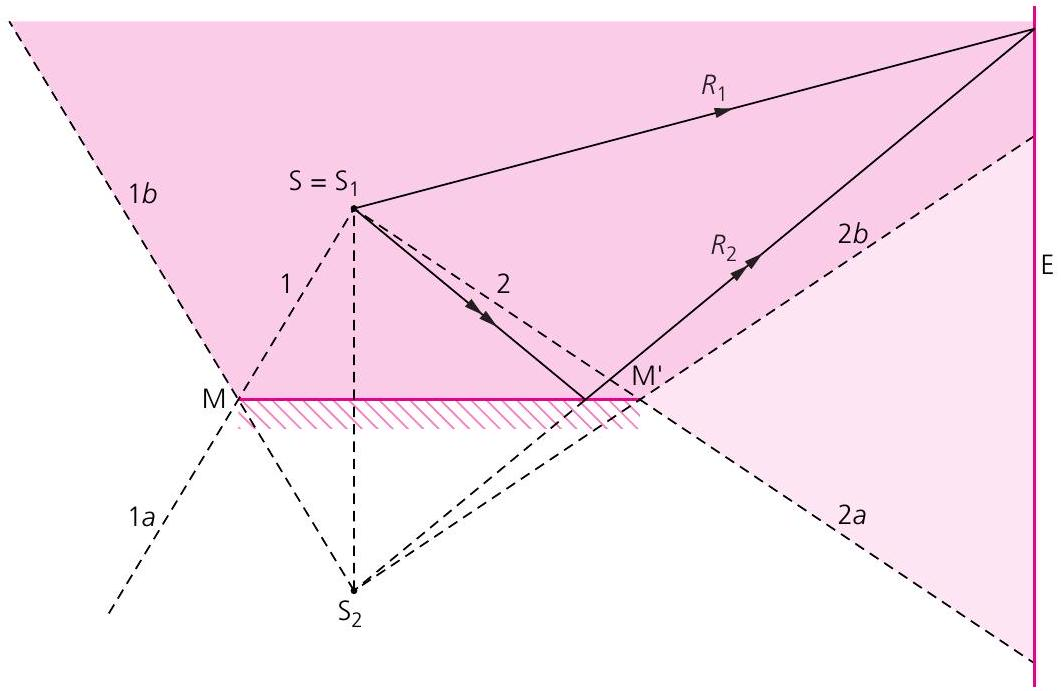
\includegraphics[width=0.7\textwidth]{images/op14.jpg}
\end{figure}
  \item La zone d'interférence correspond à la région où les deux sous-faisceaux se recouvrent (indiquée en sombre sur la figure).

  \item Les deux sous-faisceaux sont coniques de sommets $S_1 \equiv S$ et $S_2$ (image de S par le miroir). Les deux sources virtuelles sont distantes de $2a$ parallèlement à l'écran. Leur distance à l'écran est $(\ell + d)$.

  \item On applique le résultat des trous de Young :
  \[
  I(x) = I_0\!\left[1+\cos\!\left(2\pi\,\frac{2a}{\lambda(\ell+d)}\,x\right)\right]
  \]
  On observe des franges brillantes et sombres d'intensité continûment variable sur la partie de l'écran où les deux sous-faisceaux se croisent.
\end{enumerate}
\end{boitecorrige}

\subsection*{Exercice 9 - Biprisme de Fresnel en Lumière Blanche \niveau{\difficile}}

\begin{boiteexercice}
On considère un biprisme d'angle au sommet $\alpha$ (avec $\alpha$ petit) et d'indice $n = 1{,}5$. Le biprisme est éclairé par une source lumineuse ponctuelle S. On observe la figure d'interférences sur un écran à la distance $L = 3\;\text{m}$ de son sommet. La source, à la distance $D = 2\;\text{cm}$ du sommet, émet de la lumière blanche ($400\;\text{nm} < \lambda < 750\;\text{nm}$).
\begin{figure}[H]
\centering
\includegraphics[width=0.8\textwidth]{images/op22.png}
\end{figure}
\begin{enumerate}
  \item Rappeler les caractéristiques de la figure d'interférence en lumière monochromatique (largeur de la zone d'interférence et nombre de franges sombres).
  \item Combien de cannelures sombres observe-t-on au point M en lumière blanche ? Faire l'application numérique pour $x = 10\;\text{mm}$.
\end{enumerate}
\end{boiteexercice}

\begin{boitecorrige}
\begin{enumerate}
\item \textbf{Lumière monochromatique.} Le biprisme crée deux sources virtuelles $S_1$ et $S_2$ symétriques par rapport à S.
\begin{figure}[H]
\centering
\includegraphics[width=0.8\textwidth]{images/op23.png}
\end{figure}
La déviation d'un prisme de petit angle $\alpha$ est $\beta = (n-1)\alpha$. Les sources virtuelles sont séparées de :
\[
a = S_1 S_2 = 2(n-1)\alpha D
\]
\begin{figure}[H]
\centering
\includegraphics[width=0.8\textwidth]{images/op24.png}
\end{figure}
La largeur de la zone d'interférence est $d = 2(n-1)\alpha L$. L'interfrange est :
\[
i = \frac{\lambda(D+L)}{a} = \frac{\lambda(D+L)}{2(n-1)\alpha D}
\]
Le nombre de franges sombres est $N \approx d/i$.

\item \textbf{Lumière blanche --- cannelures sombres.} La différence de marche au point M(x) est :
\[
\delta(M) = \frac{a\,x}{D+L} = \frac{2(n-1)\alpha D\,x}{D+L}
\]
Les cannelures sombres correspondent aux longueurs d'onde éteintes vérifiant $\delta = (2k+1)\lambda/2$, soit :
\[
\lambda_k = \frac{2\delta(M)}{2k+1}
\]
La condition pour que $\lambda_k$ soit dans le visible ($\lambda_v = 400\;\text{nm}$, $\lambda_r = 750\;\text{nm}$) donne :
\[
\frac{2\delta(M)}{(2k+1)\lambda_r} \leq 1 \leq \frac{2\delta(M)}{(2k+1)\lambda_v}
\quad\Longrightarrow\quad
\frac{\delta(M)}{\lambda_r} - \frac{1}{2} \leq k \leq \frac{\delta(M)}{\lambda_v} - \frac{1}{2}
\]
\textbf{A.N.} Pour $x = 10\;\text{mm}$, avec les valeurs de l'énoncé on trouve $15 \leq k \leq 28$, soit \textbf{14 cannelures sombres}.
\end{enumerate}
\end{boitecorrige}

\subsection*{Exercice 10 - Coin d'air et cohérence temporelle \niveau{\moyen}}

\begin{boiteexercice}
Une onde lumineuse monochromatique plane de longueur d'onde $\lambda_0$ rencontre un coin de verre d'indice $n$ dont les faces font un angle $\alpha$ très petit. Le plan d'incidence est perpendiculaire à l'arête du coin, et l'angle d'incidence est $i$.
\begin{enumerate}
  \item Déterminer l'interfrange $\Delta x$ de la figure d'interférence obtenue par réflexion sur les faces de la lame lorsque $i = 0$.
  \item La source émet une lumière de spectre de largeur $\Delta\lambda$ centré sur $\lambda$. La longueur de cohérence est $L = \lambda^2/\Delta\lambda$. Les franges disparaissent quand la différence de marche dépasse $L$. Calculer $\alpha$ et la finesse $\lambda/\Delta\lambda$ si les franges disparaissent à la distance $l = 8\;\text{cm}$ du sommet.

Données : $\lambda = 0{,}55\;\mu\text{m}$, $i = 0$, $\Delta x = 0{,}21\;\text{mm}$, $n = 1{,}5$.
\end{enumerate}
\begin{figure}[H]
\centering
\includegraphics[width=0.7\textwidth]{images/op26.png}
\end{figure}
\end{boiteexercice}

\begin{boitecorrige}
\begin{enumerate}
  \item L'intensité lumineuse pour le coin de verre à incidence normale s'écrit :
  \[
  I(x) \approx \frac{I_0}{2}(1+\cos(2kn\alpha x))
  \]
  L'interfrange est donc :
  \[
  \Delta x = \frac{\lambda}{2n\alpha}
  \]

  \item \textbf{A.N.} $\alpha = \dfrac{\lambda}{2n\Delta x} = \dfrac{0{,}55\times10^{-6}}{2\times1{,}5\times0{,}21\times10^{-3}} = 8{,}7\times10^{-4}\;\text{rad}$.

  À la distance $l$ du sommet, la différence de marche est $\delta \approx 2nl\alpha$. Quand les franges disparaissent : $\delta = L = \lambda^2/\Delta\lambda$. L'ordre d'interférence correspondant est $P_l = \delta/\lambda = \lambda/\Delta\lambda$, soit :
  \[
  \frac{\Delta\lambda}{\lambda} = \frac{\lambda}{2nl\alpha} = \frac{\Delta x}{l} = \frac{0{,}21\;\text{mm}}{80\;\text{mm}} = 2{,}6\times10^{-3}
  \]
  La finesse est $\lambda/\Delta\lambda \approx 385$.
\end{enumerate}
\end{boitecorrige}

\subsection*{Exercice 11 - Les anneaux de Newton \niveau{\moyen}}

\begin{boiteexercice}
On considère le dispositif des anneaux de Newton. On utilise une lentille plan-convexe de rayon $R$ et d'angle d'ouverture $\theta$, dont la face courbe repose en O sur un plan de verre $Ox$. Il existe entre le plan et la lentille une lame d'air d'épaisseur $e(x)$ variable, avec $e(0) = 0$. On suppose $e \ll R$. Une source monochromatique étendue éclaire la lentille en incidence normale.
\begin{figure}[H]
\centering
\includegraphics[width=0.8\textwidth]{images/op27.png}
\end{figure}
\begin{enumerate}
  \item Rappeler quelles ondes interférent et préciser le lieu de localisation des franges.
  \item Calculer la différence de marche $\delta(x)$.
  \item Exprimer $e(x)$ en fonction de $x$. Décrire la figure d'interférence. Quel aspect a la frange centrale ?
\end{enumerate}
\end{boiteexercice}

\begin{boitecorrige}
\begin{enumerate}
  \item Les rayons qui interférent sont : $R_1$, directement réfléchis par la face courbe de la lame d'air (face courbe de la lentille), et $R_2$, réfractés dans la lame d'air puis réfléchis par la face plane. Les rayons se coupent sur la face courbe : les franges sont localisées sur la lentille (en pratique, sur le plan $Ox$ car $e$ est très petit).

  \item $R_2$ parcourt $2e(x)$ dans l'air et subit une réflexion d'un milieu d'indice 1 vers un milieu d'indice $n > 1$ : déphasage $\pi$ équivalent à $\lambda/2$. Donc :
  \[
  \delta = 2e(x) + \frac{\lambda}{2}
  \]

  \item La lentille est une portion de sphère : $R^2 = x^2 + (R-e)^2$. Avec $e \ll R$ :
  \[
  e \approx \frac{x^2}{2R}
  \]
  L'intensité est :
  \[
  I(x) = I_0\!\left(1 - \cos\!\left(\frac{2\pi x^2}{\lambda R}\right)\right)
  \]
  Les zones d'égale intensité sont des cercles concentriques. Les franges sombres ont pour rayons $x_k = \sqrt{k R \lambda}$ avec $k$ entier. Les franges brillantes ont $x_k = \sqrt{(k+1/2)R\lambda}$. La frange centrale est sombre.
\end{enumerate}
\end{boitecorrige}

\section{Interféromètre de Michelson}

\subsection*{Exercice 12 - Franges de lames minces au Michelson \niveau{\difficile}}

\begin{boiteexercice}
Dans l'interféromètre de Michelson (séparatrice G infiniment mince), la source S est étendue et monochromatique ($\lambda = 0{,}5\;\mu\text{m}$).
\begin{enumerate}
  \item Depuis la position de référence ($IK_1 = IK_2$), on déplace $M_2$ de 1\,cm selon $x$. On observe dans le plan focal image d'une lentille $L$. Qu'observe-t-on ? Quelle est la variation de l'ordre d'interférence au centre si l'on place sur l'un des bras une lame mince d'épaisseur $7{,}5\;\mu\text{m}$ et d'indice $n = 1{,}5$ ?
  \item On revient à la position $IK_1 = IK_2$ et on fait pivoter $M_2$ d'un angle $\alpha$ très faible autour d'un axe passant par $K_2$. Qu'observe-t-on sur $M_1$ ? Exprimer l'éclairement en un point P de $M_1$ tel que $K_1 P = X$. Que vaut l'interfrange $i^*$ ?
\end{enumerate}
\begin{figure}[H]
\centering
\includegraphics[width=0.4\textwidth]{images/op30.png}
\end{figure}
\end{boiteexercice}

\begin{boitecorrige}
\begin{enumerate}
  \item Le système est équivalent à une lame d'air à faces parallèles d'épaisseur $e = 1\;\text{cm}$. Avec une source étendue, on observe des \textbf{anneaux} (franges d'égale inclinaison) dans le plan focal de $L$. La différence de marche est $\delta = 2e\cos i$. L'ordre au centre vaut $p_{\text{centre}} = 2e/\lambda = 2\times10^{-2}/(5\times10^{-7}) = 40\,000$.

  Avec la lame mince d'épaisseur $e'$ et d'indice $n$ : la variation d'ordre au centre est
  \[
  |\Delta p_{\text{centre}}| = \frac{2e'(n-1)}{\lambda} = \frac{2\times7{,}5\times10^{-6}\times(1{,}5-1)}{5\times10^{-7}} = 15
  \]
  Ainsi, 15 anneaux disparaissent (ou apparaissent) au centre.

  \item L'ensemble se comporte comme un coin d'air d'angle $\alpha$ dont l'arête passe par $K_1$. On observe des \textbf{franges d'égale épaisseur} (franges rectilignes parallèles). L'épaisseur de lame équivalente en un point $P$ tel que $K_1 P = X$ est $e = \alpha X$. L'éclairement est :
  \[
  I = 2I_0\!\left[1+\cos\!\left(\frac{4\pi\alpha X}{\lambda}\right)\right]
  \]
  L'interfrange est :
  \[
  i^* = \frac{\lambda}{2\alpha}
  \]
\end{enumerate}
\end{boitecorrige}

\subsection*{Exercice 13 - Réseau de diffraction : devise spectrale \niveau{\moyen}}

\begin{boiteexercice}
Un réseau de diffraction possède $N = 600$ traits par millimètre et une largeur utile $L = \qty{2}{cm}$.
\begin{enumerate}
  \item Calculer le pas $p$ du réseau.
  \item Pour la raie verte du mercure ($\lambda = \qty{546}{nm}$), déterminer l'angle $\theta$ de diffraction à l'ordre $m=1$.
  \item Calculer le pouvoir de résolution théorique $\mathcal{R}$ à l'ordre 1, puis en déduire la plus petite différence de longueurs d'onde $\Delta\lambda$ résolvable autour de \qty{546}{nm}.
  \item Application : le mercure émet un doublet jaune ($\lambda_1 = 577{,}0\;\text{nm}$ et $\lambda_2 = 579{,}1\;\text{nm}$). Le réseau peut-il séparer ce doublet à l'ordre 1 ?
\end{enumerate}
\end{boiteexercice}

\begin{boitecorrige}
\textbf{1.} Pas du réseau : $p = 1/N = 1/600\;\text{mm} \approx 1{,}667\;\mu\text{m}$.

\textbf{2.} Formule du réseau : $p\sin\theta = m\lambda$ avec $m=1$.
\[
\sin\theta = \frac{\lambda}{p} = \frac{546\times10^{-9}}{1{,}667\times10^{-6}} \approx 0{,}328 \implies \theta \approx 19{,}1^\circ
\]

\textbf{3.} Pouvoir de résolution à l'ordre $m$ : $\mathcal{R} = mN_\text{traits}$. Le nombre total de traits éclairés est $N_\text{traits} = N\times L = 600 \times 20 = 12000$. Donc :
\[
\mathcal{R} = 1 \times 12000 = 12000
\]
Plus petite différence résolvable :
\[
\Delta\lambda_\text{min} = \frac{\lambda}{\mathcal{R}} = \frac{546}{12000} \approx 0{,}046\;\text{nm}
\]

\textbf{4.} L'écart du doublet est $\Delta\lambda = 579{,}1 - 577{,}0 = 2{,}1\;\text{nm} \gg \Delta\lambda_\text{min}$. Oui, le réseau sépare le doublet à l'ordre 1 (et même à un ordre bien plus faible).
\reponse{$\theta \approx 19{,}1^\circ$, $\mathcal{R} = 12000$, $\Delta\lambda_\text{min} \approx 0{,}046\;\text{nm}$; le doublet est résolu.}
\end{boitecorrige}

\subsection*{Exercice 14 - Polarisation circulaire et lame quart d'onde \niveau{\moyen}}

\begin{boiteexercice}
Une lumière polarisée rectilignement selon $Ox$ traverse une lame quart d'onde dont les axes sont à $45^\circ$ de $Ox$. La longueur d'onde est $\lambda = \qty{632}{nm}$.
\begin{enumerate}
  \item Rappeler l'effet d'une lame quart d'onde sur une vibration polarisée rectilignement.
  \item Déterminer la nature de la lumière émergente.
  \item Comment modifier le dispositif pour obtenir une polarisation circulaire de sens opposé ?
\end{enumerate}
\end{boiteexercice}

\begin{boitecorrige}
\textbf{1.} Une lame quart d'onde introduit un déphasage de $\pi/2$ entre les composantes de la vibration selon les axes lent et rapide. Son épaisseur vérifie $(n_e - n_o)e = \lambda/4$.

\textbf{2.} La vibration incidente $\vec{E} = E_0\cos(\omega t)\,\hat{x}$ se décompose à parts égales sur les axes de la lame (orientés à $45^\circ$) :
\[
\vec{E}_\text{lent} = \frac{E_0}{\sqrt{2}}\cos(\omega t), \quad \vec{E}_\text{rapide} = \frac{E_0}{\sqrt{2}}\cos(\omega t)
\]
À la sortie, la composante rapide est en avance de $\pi/2$ :
\[
\vec{E}_\text{sortie} = \frac{E_0}{\sqrt{2}}\left[\cos(\omega t)\,\hat{e}_\text{lent} + \cos(\omega t - \pi/2)\,\hat{e}_\text{rapide}\right] = \frac{E_0}{\sqrt{2}}\left[\cos(\omega t)\,\hat{e}_\text{lent} + \sin(\omega t)\,\hat{e}_\text{rapide}\right]
\]
Le vecteur $\vec{E}$ tourne à vitesse angulaire $\omega$ en décrivant un cercle : la lumière est \textbf{polarisée circulairement}.

\textbf{3.} Pour inverser le sens de rotation (passer de droit à gauche), il suffit de tourner la lame de $90^\circ$ (échanger les axes lent et rapide), ou d'ajouter une deuxième lame quart d'onde identique orientée à $90^\circ$ de la première.
\reponse{Lumière émergente : polarisation circulaire. Pour inverser le sens : rotation de la lame de $90^\circ$.}
\end{boitecorrige}

\subsection*{Exercice 15 - Diffraction par une ouverture circulaire \niveau{\difficile}}

\begin{boiteexercice}
Un télescope a un miroir primaire de diamètre $D = \qty{50}{cm}$. On observe une étoile émettant à $\lambda = \qty{550}{nm}$.
\begin{enumerate}
  \item Rappeler l'expression du rayon angulaire $\theta_1$ du premier anneau sombre de la figure d'Airy.
  \item Calculer $\theta_1$ en radians et en secondes d'arc.
  \item Deux étoiles sont séparées angulairement par $\alpha = 0{,}5''$. Le télescope peut-il les séparer (critère de Rayleigh) ?
  \item Quel diamètre minimal faudrait-il pour résoudre un détail de $0{,}1''$ ?
\end{enumerate}
\end{boiteexercice}

\begin{boitecorrige}
\textbf{1.} Le premier zéro de la fonction d'Airy $J_1(x)/x$ est à $x = 1{,}22\,\pi$, soit :
\[
\theta_1 = \frac{1{,}22\,\lambda}{D}
\]

\textbf{2.} Application numérique :
\[
\theta_1 = \frac{1{,}22\times 550\times10^{-9}}{0{,}50} = 1{,}342\times10^{-6}\;\text{rad}
\]
\[
\theta_1 = \frac{1{,}342\times10^{-6}\times 180\times 3600}{\pi} \approx 0{,}277''
\]

\textbf{3.} Critère de Rayleigh : deux sources sont résolues si leur séparation angulaire $\alpha \geq \theta_1$. Ici $\alpha = 0{,}5'' > 0{,}277''$ : \textbf{oui}, le télescope résout les deux étoiles.

\textbf{4.} Pour résoudre $0{,}1'' = 0{,}1\times\pi/(180\times 3600) = 4{,}85\times10^{-7}\;\text{rad}$ :
\[
D_\text{min} = \frac{1{,}22\,\lambda}{\alpha} = \frac{1{,}22\times 550\times10^{-9}}{4{,}85\times10^{-7}} \approx 1{,}38\;\text{m}
\]
\reponse{$\theta_1 \approx 0{,}277''$, séparation possible pour $\alpha = 0{,}5''$ ; $D_\text{min} \approx 1{,}38\;\text{m}$ pour $0{,}1''$.}
\end{boitecorrige}

\subsection*{Exercice 16 - Trous d'Young en lumière non monochromatique \niveau{\difficile}}

\begin{boiteexercice}
On réalise une expérience de trous d'Young avec une source émettant deux longueurs d'onde $\lambda_1 = 589{,}0\;\text{nm}$ et $\lambda_2 = 589{,}6\;\text{nm}$ (doublet du sodium). Les fentes sont distantes de $a = 0{,}4\;\text{mm}$ et l'écran est à $D = 1{,}2\;\text{m}$.
\begin{enumerate}
  \item Calculer les interfranges $i_1$ et $i_2$ correspondant à chaque longueur d'onde.
  \item À partir de quelle position $x_k$ sur l'écran observe-t-on la première coïncidence des franges brillantes des deux longueurs d'onde ?
  \item En déduire la longueur de cohérence $\ell_c$ et le temps de cohérence $\tau_c$ du doublet.
\end{enumerate}
\end{boiteexercice}

\begin{boitecorrige}
\textbf{1.} Interfrange : $i = \lambda D/a$.
\[
i_1 = \frac{589{,}0\times10^{-9}\times 1{,}2}{0{,}4\times10^{-3}} \approx 1{,}767\;\text{mm}, \quad i_2 = \frac{589{,}6\times10^{-9}\times 1{,}2}{0{,}4\times10^{-3}} \approx 1{,}769\;\text{mm}
\]

\textbf{2.} Les franges brillantes coïncident quand $k_1 i_1 = k_2 i_2$ avec $k_1 \neq k_2$ (première coïncidence : $k_2 = k_1 + 1$). On cherche le plus petit $k$ tel que :
\[
k i_1 = (k+1) i_2 \quad\Longrightarrow\quad k(i_1-i_2) = i_2
\]
\[
k = \frac{i_2}{i_1 - i_2} = \frac{1{,}769}{1{,}769 - 1{,}767} \approx 884{,}5
\]
Position de la première coïncidence :
\[
x_k = k\,i_1 \approx 884 \times 1{,}767 \approx 1{,}56\;\text{m}
\]

\textbf{3.} La longueur de cohérence est la différence de marche correspondante :
\[
\ell_c = x_k\cdot\frac{a}{D} = 1{,}56 \times \frac{0{,}4\times10^{-3}}{1{,}2} \approx 0{,}52\;\text{mm}
\]
Temps de cohérence :
\[
\tau_c = \frac{\ell_c}{c} = \frac{0{,}52\times10^{-3}}{3\times10^8} \approx 1{,}7\;\text{ps}
\]
\reponse{$i_1 \approx 1{,}767\;\text{mm}$, $i_2 \approx 1{,}769\;\text{mm}$ ; $\ell_c \approx 0{,}52\;\text{mm}$, $\tau_c \approx 1{,}7\;\text{ps}$.}
\end{boitecorrige}

\subsection*{Exercice 17 - Polariseurs croisés et lame demi-onde \niveau{\moyen}}

\begin{boiteexercice}
Une lumière naturelle d'intensité $I_0$ traverse un polariseur $P_1$ (vertical), puis une lame demi-onde dont l'axe fait un angle $\alpha$ avec la verticale, puis un polariseur $P_2$ (horizontal, donc croisé avec $P_1$).
\begin{enumerate}
  \item Donner l'intensité après $P_1$.
  \item Décrire l'effet de la lame demi-onde sur la direction de polarisation.
  \item Calculer l'intensité finale $I_s$ après $P_2$ en fonction de $I_0$ et $\alpha$.
  \item Pour quelle valeur de $\alpha$ l'intensité transmise est-elle maximale ?
\end{enumerate}
\end{boiteexercice}

\begin{boitecorrige}
\textbf{1.} Lumière naturelle : $P_1$ transmet $I_0/2$.

\textbf{2.} Une lame demi-onde introduit un déphasage de $\pi$ entre les axes lent et rapide. Une vibration polarisée selon un angle $\alpha$ par rapport à l'axe rapide ressort symétrisée par rapport à cet axe : la nouvelle direction de polarisation fait l'angle $-\alpha$ (au lieu de $+\alpha$) avec l'axe rapide. Soit un angle total $2\alpha$ entre incident et émergent.

\textbf{3.} Après $P_1$ (vertical) : polarisation verticale. La lame demi-onde la fait pivoter de $2\alpha$ (par rapport à la verticale). $P_2$ est horizontal : l'intensité transmise par $P_2$ est $I\cos^2(90^\circ - 2\alpha) = I\sin^2(2\alpha)$ :
\[
I_s = \frac{I_0}{2}\sin^2(2\alpha)
\]

\textbf{4.} Maximum pour $\sin^2(2\alpha) = 1$, soit $2\alpha = 90^\circ$ ou $\alpha = 45^\circ$ :
\[
I_{s,\max} = \frac{I_0}{2}
\]
\reponse{$I_s = (I_0/2)\sin^2(2\alpha)$ ; maximum pour $\alpha = 45^\circ$, $I_{s,\max} = I_0/2$.}
\end{boitecorrige}

\subsection*{Exercice 18 - Interféromètre de Michelson : anneaux d'égale inclinaison \niveau{\difficile}}

\begin{boiteexercice}
Un interféromètre de Michelson réglé en lame d'air (épaisseur $e = 0{,}2\;\text{mm}$) est éclairé par une source étendue de longueur d'onde $\lambda = 546\;\text{nm}$.
\begin{enumerate}
  \item Donner l'expression de la différence de marche $\delta$ en fonction de l'angle d'incidence $i$.
  \item Calculer le rayon angulaire du $k$-ième anneau brillant.
  \item Calculer le nombre d'anneaux visibles dans un champ angulaire de $10^\circ$.
  \item Que se passe-t-il si on diminue $e$ vers 0 ?
\end{enumerate}
\end{boiteexercice}

\begin{boitecorrige}
\textbf{1.} Pour le Michelson en lame d'air :
\[
\delta = 2e\cos i
\]

\textbf{2.} Anneaux brillants : $\delta = k\lambda$, soit $\cos i_k = k\lambda/(2e)$. Pour $i$ petit, $\cos i \approx 1 - i^2/2$ :
\[
i_k \approx \sqrt{\frac{2(2e - k\lambda)}{2e}} = \sqrt{2\left(1 - \frac{k\lambda}{2e}\right)}
\]
L'ordre maximal $k_\text{max}$ correspond à $i=0$ : $k_\text{max} = 2e/\lambda = 2\times 0{,}2\times10^{-3}/546\times10^{-9} \approx 733$.

\textbf{3.} Pour $i = 10^\circ = 0{,}174\;\text{rad}$, $\cos i \approx 0{,}985$ :
\[
k_\text{min} = \frac{2e\cos i}{\lambda} = \frac{2\times 0{,}2\times10^{-3}\times 0{,}985}{546\times10^{-9}} \approx 722
\]
Nombre d'anneaux visibles : $k_\text{max} - k_\text{min} \approx 733 - 722 = 11$ anneaux.

\textbf{4.} Quand $e \to 0$, $k_\text{max} \to 0$ : les anneaux s'écartent vers l'extérieur et sortent du champ. À $e = 0$ (contact optique), le champ est uniforme (teinte plate).
\reponse{$\delta = 2e\cos i$ ; environ 11 anneaux dans un champ de $10^\circ$ ; les anneaux s'écartent quand $e\to 0$.}
\end{boitecorrige}

\subsection*{Exercice 19 - Spectre cannelé d'une lame mince \niveau{\moyen}}

\begin{boiteexercice}
Une lame de verre d'épaisseur $e = 0{,}5\;\text{mm}$ et d'indice $n = 1{,}5$ est éclairée en lumière blanche. On observe le spectre de la lumière transmise à l'aide d'un spectromètre.
\begin{enumerate}
  \item Donner l'expression de la différence de marche entre les rayons réfléchis deux fois et ceux qui traversent directement.
  \item Quelles longueurs d'onde sont éteintes (cannelures sombres) ?
  \item Calculer les deux premières longueurs d'onde éteintes dans le visible ($400$-$700\;\text{nm}$).
\end{enumerate}
\end{boiteexercice}

\begin{boitecorrige}
\textbf{1.} Différence de marche en transmission : $\delta = 2ne$ (la réflexion sur le verre n'introduit pas de déphasage supplémentaire en transmission).

\textbf{2.} Cannelures sombres (interférences destructives) : $\delta = (2k+1)\lambda/2$, soit :
\[
\lambda_k = \frac{2ne}{k+\frac{1}{2}} = \frac{4ne}{2k+1}, \quad k = 0, 1, 2, \ldots
\]

\textbf{3.} Application numérique : $4ne = 4\times 1{,}5 \times 0{,}5\times10^{-3} = 3\times10^{-3}\;\text{m} = 3000\;\mu\text{m}$.
\begin{itemize}[nosep]
  \item $k=4$ : $\lambda = 3000/9 \approx 333\;\text{nm}$ (UV)
  \item $k=5$ : $\lambda = 3000/11 \approx 273\;\text{nm}$ (UV, hors visible)
\end{itemize}
Pour le visible ($400$-$700\;\text{nm}$) : $400 \leq 3000/(2k+1) \leq 700$, soit $4{,}3 \leq 2k+1 \leq 7{,}5$, donc $2k+1 \in \{5, 7\}$, soit $k=2$ ($\lambda = 600\;\text{nm}$, jaune-orange) et $k=3$ ($\lambda \approx 428\;\text{nm}$, violet).
\reponse{Cannelures visibles : $\lambda \approx 600\;\text{nm}$ et $\lambda \approx 428\;\text{nm}$.}
\end{boitecorrige}

\subsection*{Exercice 20 - Réseau blazé et ordre de diffraction \niveau{\difficile}}

\begin{boiteexercice}
Un réseau blazé possède 1200 traits/mm, et est éclairé en incidence normale. L'angle de blaze est $\theta_b = 20^\circ$.
\begin{enumerate}
  \item Calculer le pas $p$.
  \item Déterminer la longueur d'onde de blaze à l'ordre $m=1$.
  \item Pour cette longueur d'onde, calculer l'angle de diffraction.
  \item Comparer l'efficacité du réseau blazé à celle d'un réseau classique (non blazé).
\end{enumerate}
\end{boiteexercice}

\begin{boitecorrige}
\textbf{1.} Pas : $p = 1/1200\;\text{mm} \approx 833\;\text{nm}$.

\textbf{2.} Longueur d'onde de blaze à l'ordre $m$ : $\lambda_b = 2p\sin\theta_b / m$.
\[
\lambda_b = 2\times 833\times10^{-9}\times \sin(20^\circ) \approx 2\times 833\times10^{-9}\times 0{,}342 \approx 570\;\text{nm}
\]

\textbf{3.} L'angle de diffraction pour $\lambda_b$ à l'ordre 1 vérifie $p\sin\theta = \lambda_b$ :
\[
\sin\theta = \frac{\lambda_b}{p} = \frac{570}{833} \approx 0{,}684 \implies \theta \approx 43{,}1^\circ
\]
C'est bien l'angle spéculaire par rapport à la face blazée ($\theta = 2\theta_b \approx 40^\circ$ environ, l'écart vient des approximations).

\textbf{4.} Le réseau blazé concentre l'énergie dans l'ordre $m=1$ à la longueur d'onde $\lambda_b$ (efficacité $\sim 80\%$), alors qu'un réseau classique (sinusoïdal) répartit l'énergie entre plusieurs ordres (efficacité $\sim 30$-$40\%$ par ordre). Le réseau blazé est donc beaucoup plus lumineux pour les applications spectrales.
\reponse{$p \approx 833\;\text{nm}$, $\lambda_b \approx 570\;\text{nm}$, $\theta \approx 43^\circ$ ; efficacité $\sim 80\%$ (vs $\sim 30$-$40\%$ sans blaze).}
\end{boitecorrige}

\newpage
\section*{Galerie d'illustrations d'optique physique}

\begin{figure}[H]
\centering
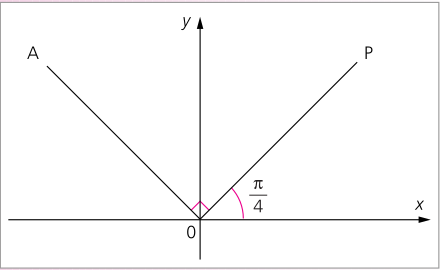
\includegraphics[width=0.7\textwidth]{images/optique_physique/op1.png}
\caption{Schéma du montage des fentes d'Young.}
\end{figure}

\begin{figure}[H]
\centering
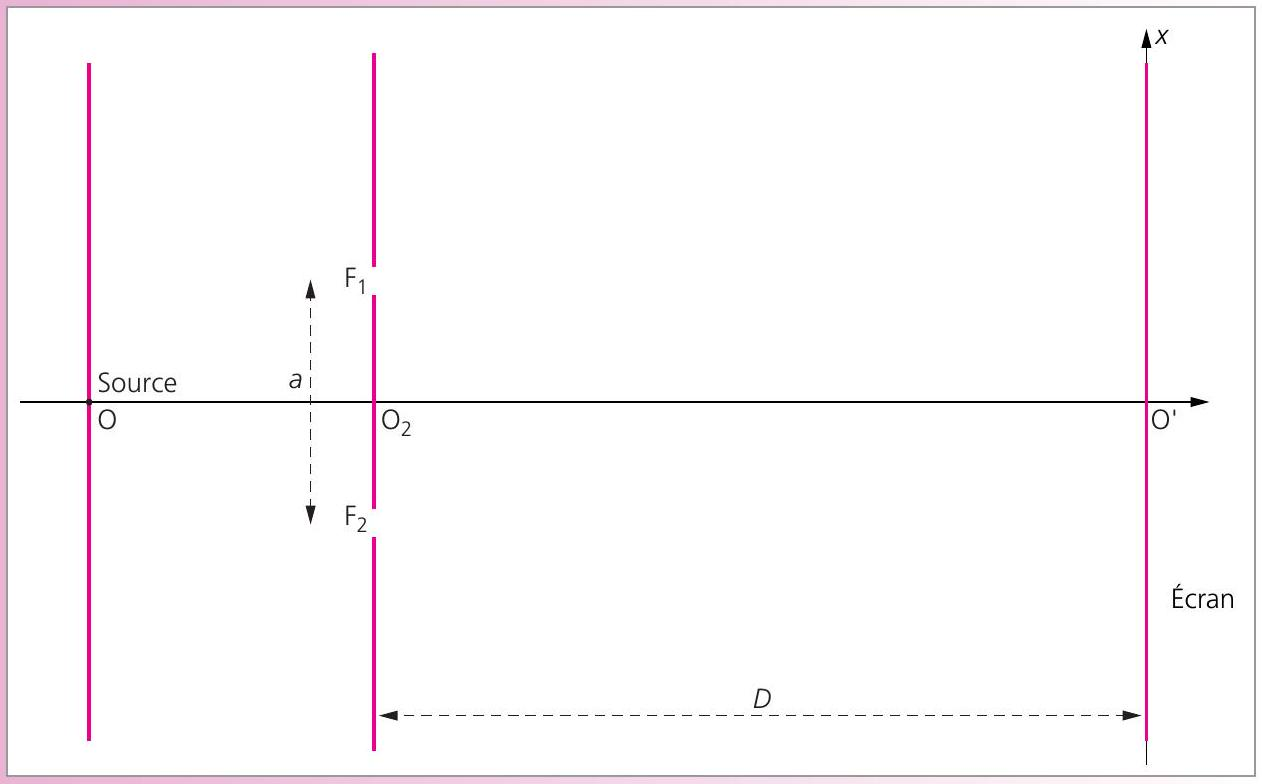
\includegraphics[width=0.7\textwidth]{images/optique_physique/op2.jpg}
\caption{Figure d'interférence observée sur l'écran.}
\end{figure}

\begin{figure}[H]
\centering
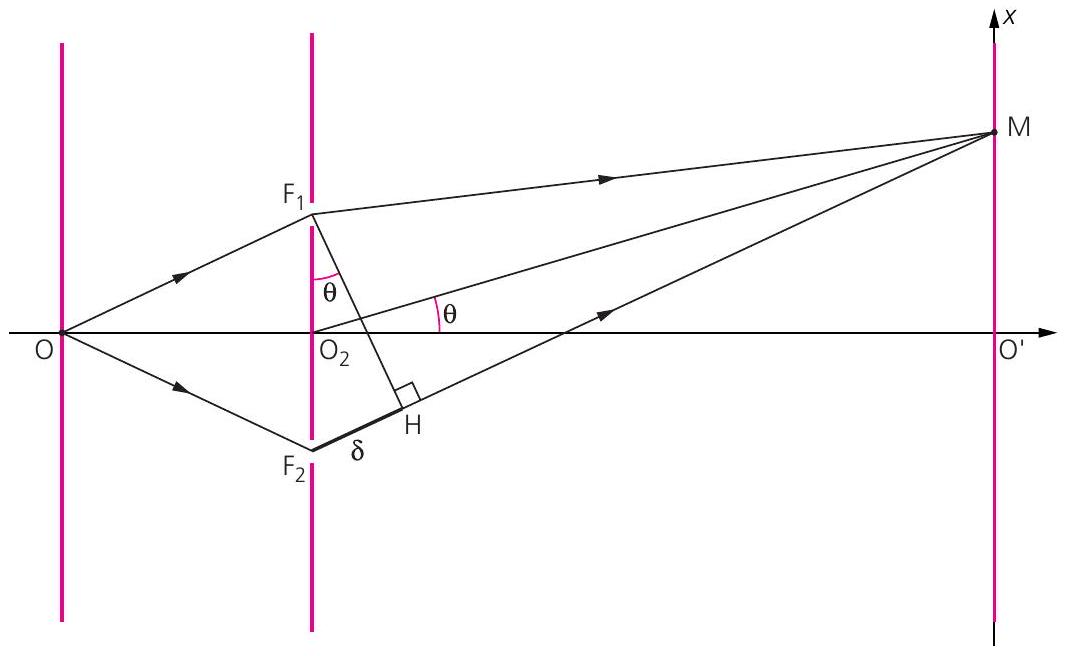
\includegraphics[width=0.7\textwidth]{images/optique_physique/op3.jpg}
\caption{Diffraction par une fente fine.}
\end{figure}

\begin{figure}[H]
\centering
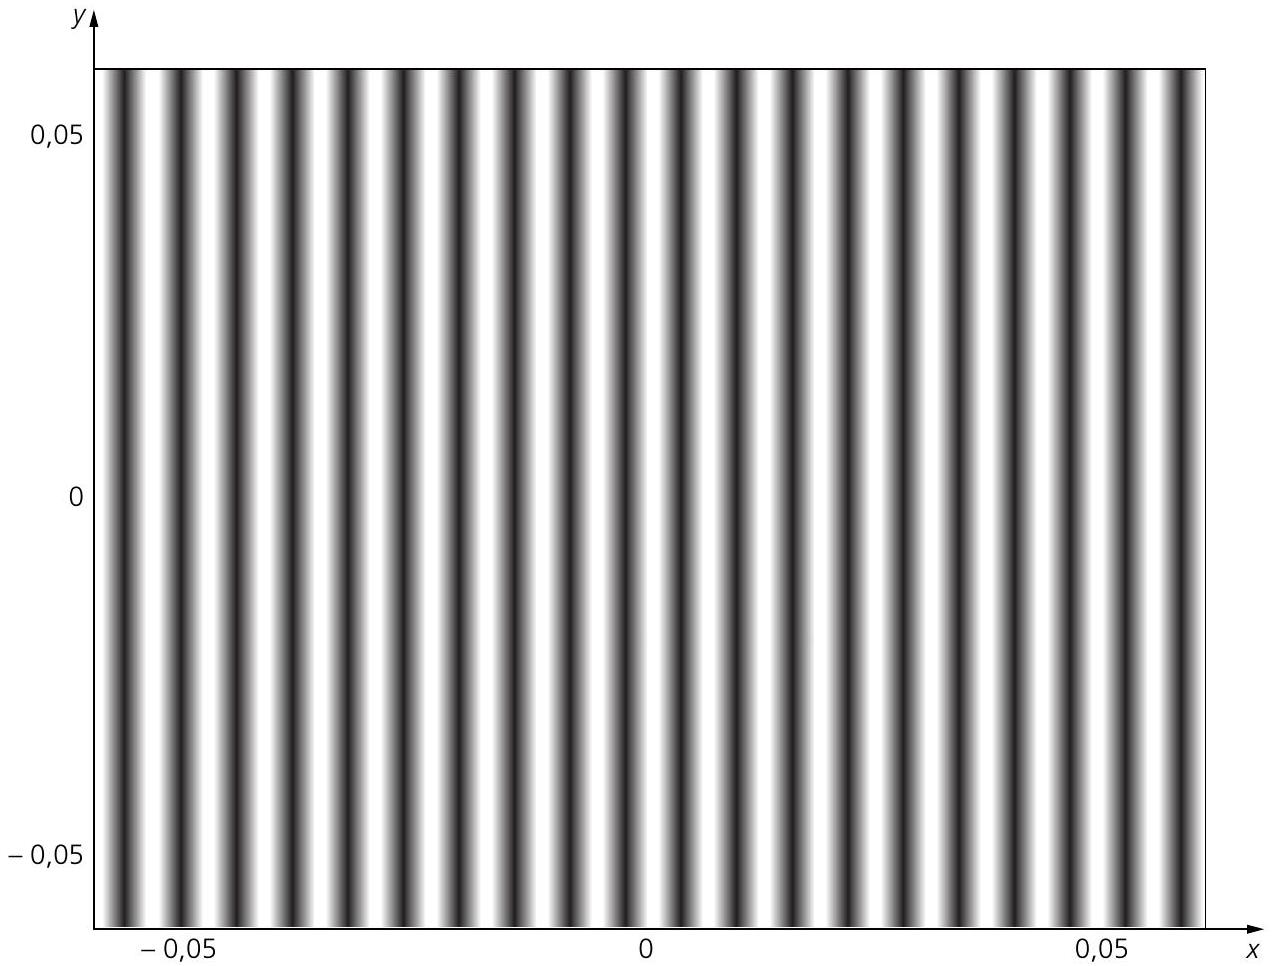
\includegraphics[width=0.7\textwidth]{images/optique_physique/op4.jpg}
\caption{Diffraction par une ouverture circulaire (figure d'Airy).}
\end{figure}

\begin{figure}[H]
\centering
\includegraphics[width=0.7\textwidth]{images/optique_physique/op5.jpg}
\caption{Réseau de diffraction : spectres d'ordres multiples.}
\end{figure}

\begin{figure}[H]
\centering
\includegraphics[width=0.7\textwidth]{images/optique_physique/op6.jpg}
\caption{Polarisation : loi de Malus.}
\end{figure}

\begin{figure}[H]
\centering
\includegraphics[width=0.7\textwidth]{images/optique_physique/op10.jpg}
\caption{Biprisme de Fresnel : géométrie.}
\end{figure}

\begin{figure}[H]
\centering
\includegraphics[width=0.7\textwidth]{images/optique_physique/op11.jpg}
\caption{Miroir de Lloyd : franges d'interférence.}
\end{figure}

\begin{figure}[H]
\centering
\includegraphics[width=0.7\textwidth]{images/optique_physique/op12.jpg}
\caption{Interféromètre de Michelson : montage.}
\end{figure}

\begin{figure}[H]
\centering
\includegraphics[width=0.7\textwidth]{images/optique_physique/op13.jpg}
\caption{Anneaux de Newton en lumière monochromatique.}
\end{figure}

\begin{figure}[H]
\centering
\includegraphics[width=0.7\textwidth]{images/optique_physique/op22.png}
\caption{Coin d'air : franges d'égale épaisseur.}
\end{figure}

\begin{figure}[H]
\centering
\includegraphics[width=0.7\textwidth]{images/optique_physique/op23.png}
\caption{Lame à faces parallèles : anneaux d'égale inclinaison.}
\end{figure}

\begin{figure}[H]
\centering
\includegraphics[width=0.7\textwidth]{images/optique_physique/op24.png}
\caption{Réseau de diffraction : spectre cannelé.}
\end{figure}

\begin{figure}[H]
\centering
\includegraphics[width=0.7\textwidth]{images/optique_physique/op26.png}
\caption{Diffraction de Fraunhofer par une fente.}
\end{figure}

\begin{figure}[H]
\centering
\includegraphics[width=0.7\textwidth]{images/optique_physique/op27.png}
\caption{Cohérence temporelle et longueur de cohérence.}
\end{figure}

\begin{figure}[H]
\centering
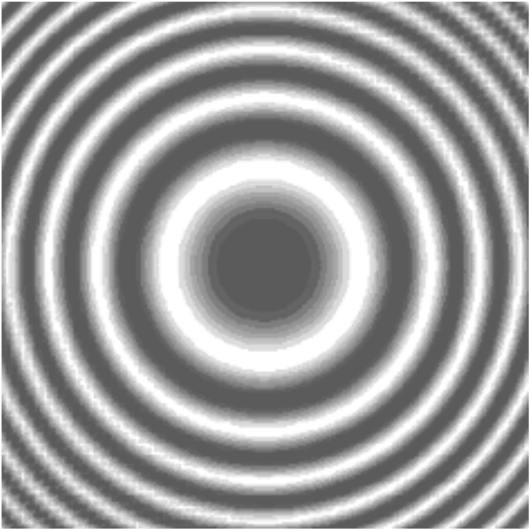
\includegraphics[width=0.7\textwidth]{images/optique_physique/op28.png}
\caption{Polarisation circulaire : composantes de la vibration.}
\end{figure}

\begin{figure}[H]
\centering
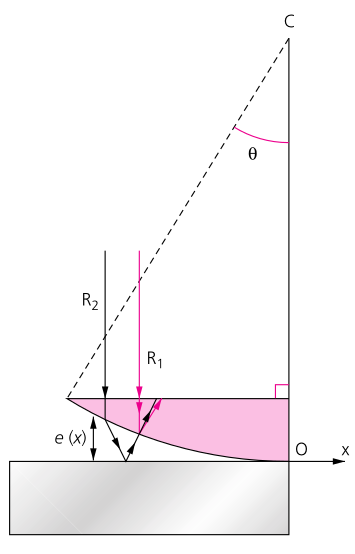
\includegraphics[width=0.7\textwidth]{images/optique_physique/op29.png}
\caption{Lame quart d'onde et demi-onde : principe.}
\end{figure}

\begin{figure}[H]
\centering
\includegraphics[width=0.7\textwidth]{images/optique_physique/op30.png}
\caption{Réseau blazé : géométrie et angle de blaze.}
\end{figure}

\ifdefined\inMainDoc\else\end{document}\fi
